\RequirePackage{plautopatch}
\documentclass[uplatex, a4paper, 14Q, dvipdfmx]{jsarticle}
\usepackage{docmute}
\usepackage{../mypackage}

\title{Bridgeland安定性}
\author{よの}
\date{\today}

\begin{document}

\maketitle

\begin{abstract}
  三角圏の$t$構造について簡単に復習し, Abel圏の安定性条件を見たあと, 三角圏の安定性条件を考える. 
\end{abstract}

\tableofcontents

\section{\texorpdfstring{$t$}{t}構造}

$\D$を三角圏, $n$を整数とする. 

\begin{definition}[拡大]
  $\D$の充満部分圏$\X, \Y$に対して
  \begin{align*}
    X \to D \to Y \to X[1] ~~(X \in \X, Y \in \Y)
  \end{align*}
  が完全三角となるような$D \in \D$のなす$\D$の部分圏を$\X$による$\Y$の拡大部分圏といい, $\X \ast \Y$と表す. 
\end{definition}

\begin{definition}[$t$構造]
  同型と直和因子で閉じた$\D$の充満加法部分圏$t^{\leq 0}, t^{\geq 0}$の対$(t^{\leq 0}, t^{\geq 0})$が次の条件を満たすとき, $(t^{\leq 0}, t^{\geq 0})$を$\D$上の$t$構造($t$-structure)という. 
  以下では, 次の記号を導入する. 
  \begin{align*}
    t^{\leq n} := t^{\leq 0}[-n], ~ t^{\geq n} := t^{\geq 0}[-n]
  \end{align*}
  \begin{enumerate}
    \item $t^{\leq 0} \perp t^{\geq 1}$ % である. つまり, $t^{\leq 0}$と$t^{\geq 0}$は直交する. 
    \item $\D = t^{\leq 0} \ast t^{\geq 1}$
    \item $t^{\leq 0} \subset t^{\leq 1}$かつ$t^{\geq 1} \supset t^{\geq 0}$
  \end{enumerate}
\end{definition}

$(t^{\leq 0}, t^{\geq 0})$を$\D$上の$t$構造とする. 

\begin{lemma}
  $t^{\leq 0} = {}^\perp (t^{\geq 1})$かつ$t^{\geq 0} = (t^{\leq -1})^\perp$である. 
\end{lemma}

\begin{corollary} \label{prop:tstr_2_out_of_3}
  完全三角$X \to Y \to Z \to X[1]$において, $X,Z \in t^{\leq 0}$のとき, $Y \in t^{\leq 0}$である. 
\end{corollary}

\begin{definition}[t構造の核]
  $\D$の充満部分圏
  \begin{align*}
    \D^\heartsuit := t^{\leq 0} \cap t^{\geq 0}
  \end{align*}
  を$t$構造の核(heart, core)という. 
\end{definition}

$t$構造の核はAbel圏の構造をもつ. 

\begin{theorem} \label{prop:heart_is_pre_abel}
  $\D$上の$t$構造$(t^{\leq 0}, t^{\geq 0})$の核$\D^\heartsuit$は前Abel圏である. 
\end{theorem}

\begin{proof}
  任意の$A,B \in \D^\heartsuit$と$f : \Hom_{\D^\heartsuit}(A,B)$に対して, ある$C \in \D$が存在して
  \begin{align} \label{dist1}
    C \xrightarrow{e} A \xrightarrow{f} B \xrightarrow{g} C[1]
  \end{align}
  は完全三角である. 
  $(t^{\leq 0}, t^{\geq 0})$は$\D$上の$t$構造なので, この$C$に対して, ある$X_C \in t^{\leq -1}$と$Y_C \in t^{\geq 0}$が存在して
  \begin{align} \label{dist2}
    X_C \xrightarrow{x_C} C[1] \xrightarrow{y_C} Y_C \to X_C[1]
  \end{align}
  は完全三角である. 
  このとき, $y_C \circ g : B \to Y_C$が$f$の余核であることを示す. 
  $y_C \circ g$に対して, ある$M \in \D$が存在して
  \begin{align} \label{dist3}
    M \xrightarrow{m} B \xrightarrow{y_C \circ g} Y_C \to M[1]
  \end{align}
  は完全三角である. 
  八面体公理より
  \begin{align} \label{dist4}
    A \xrightarrow{l} M \to X_C \to A[1]
  \end{align}
  は次の図式を可換にする完全三角である. 
  % https://q.uiver.app/#q=WzAsOCxbMSwxLCJCWy0xXSJdLFsyLDIsIllfQ1stMV0iXSxbMiwxLCJDIl0sWzMsMiwiTSJdLFszLDEsIkEiXSxbMywzLCJYX0MiXSxbMCwxLCJBWy0xXSJdLFsyLDAsIlhbLTFdIl0sWzAsMSwiKHlfQyBcXGNpcmMgZykgWy0xXSIsMl0sWzAsMiwiZ1stMV0iXSxbMiwxLCJ5X0NbLTFdIl0sWzEsM10sWzIsNF0sWzMsNV0sWzQsM10sWzEsNV0sWzYsMF0sWzcsMl1d
  \[\begin{tikzcd}
    && {X[-1]} \\
    {A[-1]} & {B[-1]} & C & A \\
    && {Y_C[-1]} & M \\
    &&& {X_C}
    \arrow["{(y_C \circ g) [-1]}"', from=2-2, to=3-3]
    \arrow["{g[-1]}", from=2-2, to=2-3]
    \arrow["{y_C[-1]}", from=2-3, to=3-3]
    \arrow[from=3-3, to=3-4]
    \arrow[from=2-3, to=2-4]
    \arrow[from=3-4, to=4-4]
    \arrow[from=2-4, to=3-4]
    \arrow[from=3-3, to=4-4]
    \arrow[from=2-1, to=2-2]
    \arrow[from=1-3, to=2-3]
  \end{tikzcd}\]
  まず, $Y_C \in \D^\heartsuit$を示す. 
  $Y_C \in t^{\geq 0}$なので, $Y_C \in t^{\leq 0}$を示せばよい. 
  \cref{dist1}において, $B \in \D^\heartsuit$かつ$A[1] \in t^{\leq -1} \subset t^{\leq 0}$なので, \cref{prop:tstr_2_out_of_3}より$C[1] \in t^{\leq 0}$である.
  \cref{dist2}において, $X[1] \in t^{\leq -2} \subset t^{\leq 0}$かつ$C[1] \in t^{\leq 0}$なので, 同様に$Y_C \in t^{\leq 0}$である. 
  よって, $Y_C \in \D^\heartsuit$である. \\
  次に, $Q \in \D^\heartsuit$と$q \in \Hom_{\D^\heartsuit}(B,Q)$が$q \circ f = 0$を満たすとする. 
  このとき, ある$q' \in \Hom_{\D^\heartsuit}(C[1],Q)$が存在して, $q' \circ g = q$である. 
  $X_C \in t^{\leq -1}$かつ$q' \circ x_C = 0$である.
  よって, ある$q'' \in \Hom_{\D^\heartsuit}(Y_C,Q)$が存在して, $q'' \circ y_C = 0$である. 
  % https://q.uiver.app/#q=WzAsNixbMCwwLCJBIl0sWzEsMCwiQiJdLFsyLDEsIkNbMV0iXSxbMywyLCJZX0MiXSxbMywwLCJRIl0sWzEsMSwiWF9DIl0sWzAsMSwiZiIsMl0sWzEsMiwiZyIsMl0sWzIsMywieV9DIiwyXSxbMSw0LCJxIl0sWzAsNCwiMCIsMCx7ImN1cnZlIjotMn1dLFsyLDQsInEnIiwyLHsic3R5bGUiOnsiYm9keSI6eyJuYW1lIjoiZGFzaGVkIn19fV0sWzUsMiwieF9DIiwyXSxbNSw0LCIwIl0sWzUsMywiMCIsMix7ImN1cnZlIjoyfV0sWzMsNCwicScnIiwyLHsic3R5bGUiOnsiYm9keSI6eyJuYW1lIjoiZGFzaGVkIn19fV1d
  \[\begin{tikzcd}
    A & B && Q \\
    & {X_C} & {C[1]} \\
    &&& {Y_C}
    \arrow["f"', from=1-1, to=1-2]
    \arrow["g"', from=1-2, to=2-3]
    \arrow["{y_C}"', from=2-3, to=3-4]
    \arrow["q", from=1-2, to=1-4]
    \arrow["0", curve={height=-12pt}, from=1-1, to=1-4]
    \arrow["{q'}"', dashed, from=2-3, to=1-4]
    \arrow["{x_C}"', from=2-2, to=2-3]
    \arrow["0", from=2-2, to=1-4]
    \arrow["0"', curve={height=12pt}, from=2-2, to=3-4]
    \arrow["{q''}"', dashed, from=3-4, to=1-4]
  \end{tikzcd}\]
  一意性を示す. 
  以上より, $y_C \circ g : B \to Y_C$は$f$の余核である. \\
  同様に, $e \circ x_C[-1] : X_C[-1] \to A$は$f$の核である. 
\end{proof}

\cref{prop:heart_is_pre_abel}より, 次の命題が成立する.

\begin{lemma} \label{prop:g_is_coker_of_f}
  任意の$f \in \Hom_{\D^\heartsuit}(A,B)$を補完する$\D$における完全三角 
  \begin{align*}
    C \xrightarrow{e} A \xrightarrow{f} B \xrightarrow{g} C[1]
  \end{align*}
  において, 次の2つが成立する.
  \begin{enumerate}
    \item $C[1] \in t^{\geq 0}$のとき, $g$は$f$の余核である.
    \item $C \in t^{\leq 0}$のとき, $e$は$f$の核である. 
  \end{enumerate}
\end{lemma}

\begin{theorem} \label{prop:heart_is_abel}
  $\D$上の$t$構造の核$\D^\heartsuit$はAbel圏である. 
\end{theorem}

\begin{proof}
  任意の$f \in \Hom_{\D^\heartsuit}(A,B)$に対して, $\Im{f} \cong \Coim{f}$が成立することを示す. 
  \cref{dist4}において, $A \in \D^\heartsuit$かつ$X_C[1] \in t^{\leq -2} \subset t^{\leq0}$より, $M \in t^{\leq 0}$である. 
  \cref{prop:g_is_coker_of_f}より, $m = \ker{y_C \circ g} = \ker{\coker{f}}$である. 
  よって, $\im{f} = m$なので, $f = m \circ l$と像経由分解できる.
  同様に, $\coim{f} = l$となっているので, $f = m \circ l$は余像経由分解でもある. 
  よって, 同型$\Im{f} \cong \Coim{f}$が存在する. 
  % https://q.uiver.app/#q=WzAsNSxbMSwxLCJBIl0sWzMsMSwiQiJdLFsyLDAsIk0iXSxbNCwyLCJZX0MiXSxbMCwwLCJYX0NbLTFdIl0sWzAsMSwiZiIsMl0sWzAsMiwibCJdLFsyLDEsIm0iXSxbMSwzLCJ5X0MgXFxjaXJjIGciXSxbNCwwLCJlIFxcY2lyYyB4X0NbLTFdIiwyXV0=
  \[\begin{tikzcd}
    {X_C[-1]} && M \\
    & A && B \\
    &&&& {Y_C}
    \arrow["f"', from=2-2, to=2-4]
    \arrow["l", from=2-2, to=1-3]
    \arrow["m", from=1-3, to=2-4]
    \arrow["{y_C \circ g}", from=2-4, to=3-5]
    \arrow["{e \circ x_C[-1]}"', from=1-1, to=2-2]
  \end{tikzcd}\]
\end{proof}

\begin{definition}[有界$t$構造]
  $\D$上の$t$構造$(t^{\leq 0}, t^{\geq 0})$は次の条件を満たすとき, $(t^{\leq 0}, t^{\geq 0})$は有界(bounded)であるという.
  \begin{align*}
    \D = \bigcup_{i,j \in \bbZ} (t^{\leq 0} \cap t^{\geq 0})
  \end{align*}
\end{definition}

\section{Abel圏上の安定性条件}

$\A$をAbel圏, $K(\A)$を$\A$上のGrothendieck群とする. 

\begin{definition}[Abel圏上の安定関数]
  群準同型$Z : K(\A) \to \bbC$は次の条件を満たすとき, $Z$を$\A$上の安定関数(stability function)という. 
  \begin{itemize}
    \item 任意の$E (\neq 0) \in \A$に対して, $Z(E) \in \bbH$である. 
    ここで
    \begin{align*}
      \bbH := \{r \exp(i \pi \phi) ~|~ r>0, 0 < \phi \leq 1 \} \subset \bbC
    \end{align*}
  \end{itemize}
  安定関数$Z$に対して, $E (\neq 0) \in \A$の位相(phase) $\phi(E)$を次の式で定義する.
  \begin{align*}
    \phi(E) := \frac{1}{\pi} \arg Z(E) \in (0,1]
  \end{align*} 
\end{definition}

\begin{definition}[半安定対象]
  $Z : K(\A) \to \bbC$を$\A$上の安定関数とする. 
  $E (\neq 0) \in \A$の任意の部分対象$A \in \A$に対して$\phi(A) \leq \phi(E)$であるとき, $E$を$Z$による半安定対象(the semistable object with respect to $Z$)という. 
\end{definition}

\begin{definition}[Harder-Narasimhanフィルトレーション]
  
\end{definition}

\section{スライス}

$\D$を三角圏とする. 

\begin{definition}[スライス]
  任意の$\phi \in \bbR$に対して, $\P(\phi)$を$\D$の充満加法部分圏とする.
  $\P = \{\P(\phi)\}_{\phi_\in \bbR}$が次の条件を満たすとき, $\P$を$\D$のスライス(slicing)という.
  $\P(\phi)$の$0$でない対象を位相$\phi$の対象という. 
  \begin{enumerate}
    \item 任意の$\phi \in \bbR$に対して, $\P(\phi+1) = \P(\phi)[1]$
    \item $\phi_1 > \phi_2$のとき, $\P(\phi_1) \perp \P(\phi_2)$
    \item 任意の$E (\neq 0) \in \D$に対して, ある実数の有限列
    \begin{align*}
      \phi_1 > \cdots > \phi_n
    \end{align*}
    と, 完全三角の列
    \[
      \begin{tikzpicture}[->,auto]
        \node (E0) at (2,0) {$0 = E_0$};
        \node (E1) at (4,0) {$E_1$};
        \node (E2) at (6,0) {$E_2$};
        \node (cdots) at (8,0) {$\cdots$};
        \node (En-1) at (10,0) {$E_{n-1}$};
        \node (En) at (12,0) {$E_n = E$};
        \node (A1) at (3,-1.5) {$A_1$};
        \node (A2) at (5,-1.5) {$A_2$};
        \node (An) at (11,-1.5) {$A_n$};
        \draw (E0) -- (E1); \draw (E1) -- (E2);
        \draw (E2) -- (cdots);
        \draw (cdots) -- (En-1);
        \draw (En-1) -- (En);
        \draw (E1) -- (A1);
        \draw[dashed] (A1) -- (E0); 
        \draw (E2) -- (A2);
        \draw[dashed] (A2) -- (E1);
        \draw (En) -- (An);
        \draw[dashed] (An) -- (En-1);  
      \end{tikzpicture}
    \]
    が存在して, 各$i$に対して, $A_i \in \P(\phi_i)$である. 
  \end{enumerate}
\end{definition}

条件(3)における完全三角の列は次のような意味で用いている. 

\begin{remark}
  % https://q.uiver.app/#q=WzAsMTMsWzAsMCwiRV8wIl0sWzEsMCwiRV8xIl0sWzIsMCwiQV8xIl0sWzMsMCwiRV8wWzFdIl0sWzEsMSwiRV8yIl0sWzIsMSwiQV8yIl0sWzMsMSwiRV8xWzFdIl0sWzEsMiwiXFxjZG90cyJdLFsyLDIsIlxcY2RvdHMiXSxbMywyLCJcXGNkb3RzIl0sWzEsMywiRV9uIl0sWzIsMywiQV9uIl0sWzMsMywiRV97bi0xfVsxXSJdLFswLDEsImZfMSJdLFsxLDIsImdfMSJdLFsyLDMsImhfMSJdLFsxLDQsImZfMiIsMl0sWzQsNSwiZ18yIl0sWzUsNiwiaF8yIl0sWzQsN10sWzcsOF0sWzgsOV0sWzcsMTAsImZfbiIsMl0sWzEwLDExLCJnX24iXSxbMTEsMTIsImhfbiJdXQ==
  \[\begin{tikzcd}
    {E_0} & {E_1} & {A_1} & {E_0[1]} \\
    & {E_2} & {A_2} & {E_1[1]} \\
    & \cdots & \cdots & \cdots \\
    & {E_n} & {A_n} & {E_{n-1}[1]}
    \arrow["{f_1}", from=1-1, to=1-2]
    \arrow["{g_1}", from=1-2, to=1-3]
    \arrow["{h_1}", from=1-3, to=1-4]
    \arrow["{f_2}"', from=1-2, to=2-2]
    \arrow["{g_2}", from=2-2, to=2-3]
    \arrow["{h_2}", from=2-3, to=2-4]
    \arrow[from=2-2, to=3-2]
    \arrow[from=3-2, to=3-3]
    \arrow[from=3-3, to=3-4]
    \arrow["{f_n}"', from=3-2, to=4-2]
    \arrow["{g_n}", from=4-2, to=4-3]
    \arrow["{h_n}", from=4-3, to=4-4]
  \end{tikzcd}\]
  を
  \[
    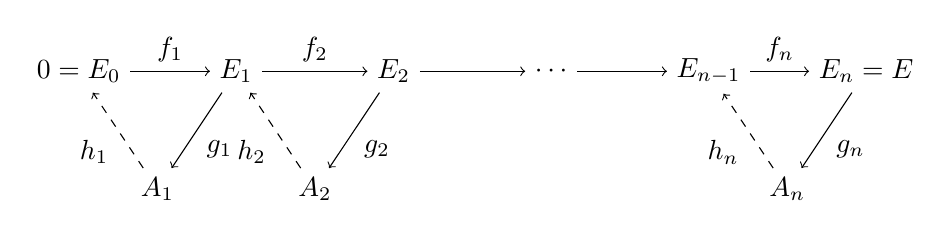
\begin{tikzpicture}[->,auto]
      \node (E0) at (2,0) {$0 = E_0$};
      \node (E1) at (4,0) {$E_1$};
      \node (E2) at (6,0) {$E_2$};
      \node (cdots) at (8,0) {$\cdots$};
      \node (En-1) at (10,0) {$E_{n-1}$};
      \node (En) at (12,0) {$E_n = E$};
      \node (A1) at (3,-1.5) {$A_1$};
      \node (A2) at (5,-1.5) {$A_2$};
      \node (An) at (11,-1.5) {$A_n$};
      \draw (E0) -- node {$f_1$} (E1); 
      \draw (E1) -- node {$f_2$} (E2);
      \draw (E2) -- (cdots);
      \draw (cdots) -- (En-1);
      \draw (En-1) -- node {$f_n$} (En);
      \draw (E1) -- node {$g_1$} (A1);
      \draw[dashed] (A1) -- node {$h_1$} (E0); 
      \draw (E2) -- node {$g_2$} (A2);
      \draw[dashed] (A2) -- node {$h_2$} (E1);
      \draw (En) -- node {$g_n$} (An);
      \draw[dashed] (An) -- node {$h_n$} (En-1);  
    \end{tikzpicture}
  \]
  と表している. 
\end{remark}

$\P$を$\D$のスライスとする. 

\begin{lemma} \label{prop:filtration_is_unique_up_to_iso}
  条件(3)における完全三角の列は同型を除いて一意である. 
\end{lemma}

\cref{prop:filtration_is_unique_up_to_iso}より, $0$でない対象から最大の位相と最小の位相という不変量が定まる. 

\begin{definition}
  任意の$E (\neq 0) \in \D$に対して
  \begin{align*}
    \phi^+_\P(E) := \phi_1,~~ \phi^-_\P(E) := \phi_n
  \end{align*}
  とする. 
  $\P$が明らかな場合は$\P$を省略する.
  また, $\{A_i\}$を$E$の半安定要素(semistable factors)という. 
\end{definition}

\begin{lemma}
  任意の$E (\neq 0) \in \D$に対して, 次の式が成立する. 
  \begin{align*}
    \phi^+_\P(E) \geq \phi^-_\P(E)
  \end{align*}
  ある$\phi \in \bbR$が存在して, $E \in \P(\phi)$となるときに等号は成立する. 
\end{lemma}

\begin{definition}
  任意の$I \subset \bbR$に対して, 各$\phi \in I$における$\P(\phi)$によって生成される$\D$の拡大で閉した部分圏を$\P(I)$とする. 
  つまり, $\P(I)$は次のように表せる. 
  \begin{align*}
    \P(I) := \{0\} \cup \{E \in \D ~|~ \phi^+(E), \phi^-(E) \in I\}
  \end{align*}
  また, 任意の$t \in \bbR$に対して, 次のような省略を用いる.
  \begin{align*}
    \P(\leq t) &:= \P((-\infty,t]) = \{0\} \cup \{E \in \D ~|~ \phi^+(E) \leq t\} \\
    \P(< t)    &:= \P((-\infty,t)) = \{0\} \cup \{E \in \D ~|~ \phi^+(E) < t\} \\
    \P(\geq t) &:= \P([t,\infty)) = \{0\} \cup \{E \in \D ~|~ \phi^-(E) \geq t\} \\
    \P(> t)    &:= \P((t,\infty)) = \{0\} \cup \{E \in \D ~|~ \phi^-(E) > t\}
  \end{align*}
\end{definition}

\begin{lemma}
  $I$を長さ$1$上の区間とする. 
  $\D$における完全三角$A \to E \to B$において, $A,E,B$は$\P(I)$の$0$でない対象とする. 
  このとき, $\phi^+(A) \leq \phi^+(E)$かつ$\phi^-(E) \leq \phi^-(B)$である. 
\end{lemma}

\begin{proof}
  $\phi^+(A) \leq \phi^+(E)$を示す. 
  ある$t \in \bbR$と$\alpha \in \bbR_{\geq 1}$を用いて, $I = [t,t+\alpha]$と表す. 
  定義より, ある$A^+ \in \P(\phi^+(A))$が存在する. 
  $A_1 \cong A^+$なので, $0$でない射$f : A^+ \to A$が存在する. \\
  $\phi^+(A) > \phi^+(E)$であると仮定する.
  定義より, $\Hom_\D(A^+,F_n) = 0$である. 
  $\Hom_\D(E,F_n) \neq 0$なので, $\Hom_\D(A^+,E) = 0$であり, $f$は$B[-1]$を経由する(らしい).
  % https://q.uiver.app/#q=WzAsMTIsWzMsMSwiQV97bi0xfSJdLFs0LDEsIkEiXSxbNCwyLCJDX24iXSxbNiwxLCJFIl0sWzUsMiwiQiJdLFs3LDEsIkVfe24tMX0iXSxbNiwyLCJGX24iXSxbMiwxLCJcXGNkb3RzIl0sWzEsMSwiQV8xIl0sWzAsMSwiQV8wIl0sWzEsMCwiQV4rIl0sWzgsMSwiXFxjZG90cyJdLFswLDFdLFsxLDJdLFsyLDAsIiIsMCx7InN0eWxlIjp7ImJvZHkiOnsibmFtZSI6ImRhc2hlZCJ9fX1dLFsxLDNdLFszLDRdLFs0LDEsIiIsMCx7InN0eWxlIjp7ImJvZHkiOnsibmFtZSI6ImRhc2hlZCJ9fX1dLFs1LDNdLFszLDZdLFs2LDUsIiIsMCx7InN0eWxlIjp7ImJvZHkiOnsibmFtZSI6ImRhc2hlZCJ9fX1dLFs3LDBdLFs4LDddLFs5LDhdLFs4LDEwXSxbMTAsOSwiIiwyLHsic3R5bGUiOnsiYm9keSI6eyJuYW1lIjoiZGFzaGVkIn19fV0sWzEwLDEsImYgKFxcbmVxIDApIl0sWzEwLDMsIjAiLDAseyJjdXJ2ZSI6LTJ9XSxbMTEsNV1d
  \[\begin{tikzcd}
    & {A^+} \\
    {A_0} & {A_1} & \cdots & {A_{n-1}} & A && E & {E_{n-1}} & \cdots \\
    &&&& {C_n} & B & {F_n}
    \arrow[from=2-4, to=2-5]
    \arrow[from=2-5, to=3-5]
    \arrow[dashed, from=3-5, to=2-4]
    \arrow[from=2-5, to=2-7]
    \arrow[from=2-7, to=3-6]
    \arrow[dashed, from=3-6, to=2-5]
    \arrow[from=2-8, to=2-7]
    \arrow[from=2-7, to=3-7]
    \arrow[dashed, from=3-7, to=2-8]
    \arrow[from=2-3, to=2-4]
    \arrow[from=2-2, to=2-3]
    \arrow[from=2-1, to=2-2]
    \arrow[from=2-2, to=1-2]
    \arrow[dashed, from=1-2, to=2-1]
    \arrow["{f (\neq 0)}", from=1-2, to=2-5]
    \arrow["0", curve={height=-12pt}, from=1-2, to=2-7]
    \arrow[from=2-9, to=2-8]
  \end{tikzcd}\]
\end{proof}

\begin{lemma}
  任意の$\phi \in \bbR$に対して, $(\P(> \phi), \P(\leq \phi+1))$と$(\P(\geq \phi), \P(< \phi+1))$は$\D$上の$t$構造である. 
\end{lemma}

\begin{proof}
  $(\P(> \phi), \P(\leq \phi+1))$が$t$構造であることを示す. \\
  まず, $\P(> \phi) \perp \P(\leq \phi)$を示す.
  任意の$E \in \P(> \phi)$と$F \in \P(\leq \phi)$に対して, $\phi^-(E) > \phi \geq \phi^+(F)$なので, $\Hom(E,F) = 0$である. \\
  次に, $\D = \P(> \phi) \ast \P(\leq \phi)$を示す. 
  $\D \supset \P(> \phi) \ast \P(\leq \phi)$は明らかなので, 逆を示す.
  任意の$E \in \D$に対して, 条件(3)の$\phi$以下と$\phi$より大きい実数で完全三角の列を分ける. 
  このとき, 次の完全三角が存在するので, $\D \subset \P(> \phi) \ast \P(\leq \phi)$である.  
  % https://q.uiver.app/#q=WzAsMyxbMCwwLCJcXFAoPiBcXHBoaSkgXFxuaSBFX3tuLTF9Il0sWzIsMCwiRSBcXGluIFxcRCJdLFsxLDEsIkFfbiBcXGluIFxcUChcXGxlcSBcXHBoaSkiXSxbMCwxXSxbMSwyXSxbMiwwLCIiLDAseyJzdHlsZSI6eyJib2R5Ijp7Im5hbWUiOiJkYXNoZWQifX19XV0=
  \[\begin{tikzcd}
    {\P(> \phi) \ni E_{n-1}} && {E \in \D} \\
    & {A_n \in \P(\leq \phi)}
    \arrow[from=1-1, to=1-3]
    \arrow[from=1-3, to=2-2]
    \arrow[dashed, from=2-2, to=1-1]
  \end{tikzcd}\]
  最後に, $\P(> \phi) \subset \P(> \phi)[-1]$を示す.
  定義より
  \begin{align*}
    \P(> \phi)[-1] = \P(\leq \phi-1) = \{0\} \cup \{E \in \D ~|~ \phi - 1 < \phi^-(E)\}
  \end{align*}
  なので, $\P(> \phi) \subset \P(> \phi)[-1]$である.
  同様に, $\P(\leq \phi)[-1] \supset \P(\leq \phi)$も示せる. \\
  以上より, $(\P(> \phi), \P(\leq \phi+1))$は$t$構造である.
\end{proof}

\begin{corollary}
  $t$構造$(\P(> \phi), \P(\leq \phi+1))$の核は$\P((\phi,\phi+1])$の部分集合である. 
  $t$構造$(\P(\geq \phi), \P(< \phi+1))$の核は$\P([\phi,\phi+1))$の部分集合である. 
\end{corollary}

\section{Bridgeland安定性}

$\D$を三角圏, $K(\D)$を$\D$のGrothendieck群とする.

\begin{definition}[三角圏上の安定性条件]
  群準同型$Z : K(\D) \to \C$と次の条件を満たす$\D$のスライス$\P$の組$\sigma = (Z,\P)$を$\D$上の安定性条件(stability condition)という.
  \begin{itemize}
    \item 任意の$E (\neq 0) \in \P(\phi)$に対して, ある$m(E) \in \bbR_{\geq 0}$が存在して, $Z(E) = m(E) \exp (i \pi \phi)$である. 
  \end{itemize}
  群準同型$Z$を安定性条件の中心電荷(central charge), $\P(\phi)$の対象を位相$\phi$の半安定対象(semistable objects with phase $\phi$), $\P(\phi)$の単純対象を位相$\phi$の安定対象(stable objects with phase $\phi$)という. 
\end{definition}

$(Z,\P)$を$\D$上の安定性条件とする. 

\begin{lemma}
  任意の$\phi \in \bbR$に対して, $\P(\phi)$はAbel圏である. 
\end{lemma}

\begin{definition}[質量]
  任意の$E (\neq 0) \in \D$に対して
  \begin{align*}
    m_\sigma(E) := \sum_i |Z(A_i)|
  \end{align*}
  を$E$の質量(mass)という.
  $\sigma$が明らかな場合は$\sigma$を省略する. 
\end{definition}

\begin{lemma}
  $E (\neq 0) \in \D$に対して, 次の式が成立する. 
  \begin{align*}
    m_\sigma(E) \geq |Z(E)|
  \end{align*}
  ある$\phi \in \bbR$が存在して, $E \in \P(\phi)$となるときに等号は成立する. 
\end{lemma}

\begin{theorem}
  次の2つは同値である. 
  \begin{enumerate}
    \item $\D$上に安定性条件を与える.
    \item $\D$上の有界$t$構造の核とHNフィルトレーションをもつその上の安定性条件を与える. 
  \end{enumerate}
\end{theorem}

\begin{proof}
  (1)から(2)を示す. 
  $\D$上の有界$t$構造の核を$\D^\heartsuit$とすると, 自然な同型$K(D^\heartsuit) \cong K(\D)$がある. 

\end{proof}

\begin{definition}[局所有限]
  
\end{definition}

\section{安定性条件のなす空間}

$\D$を三角圏とする. 

\begin{definition}[スライスと安定性条件のなす集合]
  局所有限なスライスのなす集合を$\Slice(\D)$, 局所有限な安定性条件のなす集合を$\Stab(\D)$と表す. 
\end{definition}

\begin{lemma}
  任意の$\P,\Q \in \Slice(\D)$に対して
  \begin{align*}
    d(\P,\Q) := \sup_{E (\neq 0) \in \D} \qty{\myabs{\phi^-_\P(E) - \phi^-_\Q(E)}, \myabs{\phi^+_\P(E) - \phi^+_\Q(E)}}
    \in [0,\infty) 
  \end{align*}
  は$\Slice(D)$上の距離を定める. 
\end{lemma}



\end{document}